%\dropchapter{0.4in}
\chapter{chapter 3} \label{chp:labelTitle}
%\epigraphhead[70]{\epigraph{\textit{If I could remember the names of all these particles, I'd be a botanist.}}{Enrico Fermi}}
%\undodrop

An accurate understanding of simulated events and their reconstruction is crucial for a thorough understanding of the collected data. Hence event generators such as $\Madgraph$, $\Pythia$ and $\Herwig$ play the role of hadron colliders and allow some improvement of analyzing power by using an efficient background and signal discriminator.

\section{QCD for hadron colliders} \label{sec::QCDHadron}

The event generation process in hadron colliders is arduous due to QCD activity in a widespread energy range. The phenomena of interest studied by the LHC consist of momentum transfers in a range between $50$ $\GeV$ and $5$ $\TeV$, however, the initial partons responsible for these collisions are protons with a mass of barely $0.938$ $\GeV$ \cite{}. The former energy-range results in a tiny QCD coupling such that perturbation theory can be assumed to be valid, while the incoming partons' energy range is far too low for perturbation theory to hold. Therefore throughout the consecutive steps of the event generation process some aspects can be derived exactly from the QCD Lagrangian while others are expressed using phenomenological non-perturbative models. An overview of the event generation process process, for which all separate stages will be discussed in detail further, is depicted in Figure~\ref{fig::EvtShower}.
%\textit{Is there still a part which is described by perturbative QCD? Everything is approximate no?}  --> Perturbative part is the HARD scattering!

\begin{figure}[htb]
 \centering
 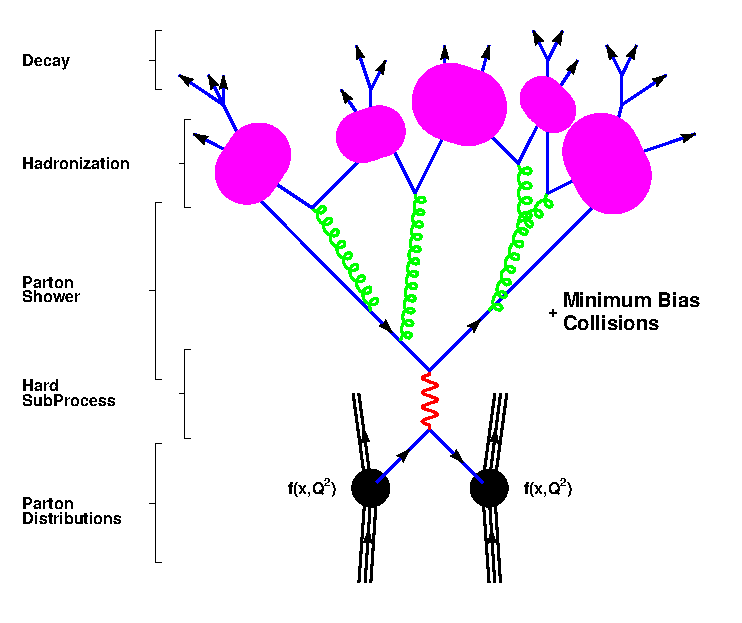
\includegraphics[width = 0.8 \textwidth]{Chapters/Chapter3/Figures/f_shg_event.eps}
 \caption{Schematical overview of the consecutive steps of the event generation process.}  \label{fig::EvtShower}
\end{figure}

\begin{myindentpar}
  \begin{description}
    \item[Parton Distribution Functions] \hfill \\
      In proton-proton collisions both incoming protons can be viewed as a collection of partons whose momentum fraction $x$ within the hadron is parametrized by the so-called parton distribution functions.
    \item[Hard scattering (or factorization?)] \hfill \\
      The perturbative process when the collision of two partons, one originating from each proton, creates high-energetic particles is defined as hard scattering. This process can be represented by a factorized product of short-and long-distance processes as discussed in Section~\ref{sec::HardScattering}.
    \item[Parton shower (or is this factorization??)] \hfill \\
      This phase of the event generation process includes the approximate higher-order corrections induced by emission of additional gluon and/or quarks, as will be explained in detail in Section~\ref{sec::PS}. Depending whether this radiation originates from the incoming or outgoing partons this is called Initial State Radiation (ISR) or Final State Radiation (FSR), respectively.
    \item[Hadronisation] \hfill \\
      Due to color confinement the collection of (receding) post-shower partons has to combine into experimentally observable color-neutral hadrons. This process, called hadronisation, is described by QCD-inspired phenomenological models as discussed in Section~\ref{sec::Hadronisation}.
    %\item[Underlying event (why is this a separate item? Doesn't show up in the schematical overview ...)] \hfill \\
  \end{description}
\end{myindentpar}

\subsection{Hard Scattering (=? Jet Fragmentation)} \label{sec::HardScattering}
Due to the internal structure of the protons, the inclusive cross section $\sigma_{h_{1}h_{2} \rightarrow X}$ cannot be calculated exactly from first principles but has to be factorized in terms of the partonic scattering cross section $\hat{\sigma}_{ab \rightarrow X}$ and the parton distribution functions $f_{a}^{h}$. Therefore, within the collinear limit~\cite{ColLimit}, the inclusive cross section for $X$-production can be written as:
%Since the hard scattering interaction occurs between two partons present in the proton, it probes the energy scale far below the mass range of the proton. In this region perturbative QCD is valid and the cross-section can be calculated from first principles (not completely true, the PDF's cannot be calculated from first principles since it concerns small momentum transfers!!) REMARK: LOW ENERGY SCALE MEANS NO PQCD!!.\\
%Within collinear factorization the cross-section of such an hard interacting event can be seen as a convolution between the partonic cross section $\hat{\sigma}$ and the long-scale parton distribution functions (PDF's) which represent the flux of the partons within the proton. (\textit{BETTER LAST SENTENCE!})\\
%The inclusive cross section of creating the final state $X$ from the hadrons $h_{1}$,$h_{2}$ can be written in terms of the partonic cross section $\hat{\sigma}_{ab \rightarrow X}$: (\textit{Still not much better.}
\\ \textit{Should check whether there is a difference between $\hat{\sigma}_{ab \rightarrow X}$ and $\hat{\sigma}(\Phi_{ab \rightarrow X},\mu^{2}_{F})$??}
\begin{equation} \label{eq::HSXS}
 \sigma_{h_{1}h_{2} \rightarrow X} =\sum_{a,b \in \{q,g\} } \int dx_{a} \int dx_{b} f_{a}^{h_{1}}(x_{a},\mu^{2}_{F}) f_{b}^{h_{2}}(x_{b},\mu^{2}_{F}) \int d\Phi_{ab \rightarrow X} \dfrac{d\hat{\sigma}(\Phi_{ab \rightarrow X},\mu^{2}_{F})}{d\Phi_{ab \rightarrow X}}
\end{equation}
As Equation~(\ref{eq::HSXS}) suggests, the hadronic cross section is actually a convolution of a perturbatively short-distance part $\hat{\sigma}_{ab \rightarrow X}$, calculable from Matrix Elements, and an approximately long-distance part, represented by the parton distribution functions (PDF). The PDF $f_{a}^{h}(x_{a},\mu_{F})$ symbolizes the probability of encountering a parton $a$ with momentum fraction $x_a$ within the hadron $h$ at the energy scale $\mu_{F}$. This factorization scale $\mu_{F}$ represents the transition from the short-distance process to the long-distance one.\\
\textit{Should the terms of the second integrand be mentioned specifically??}\\
\\
\textit{What else can/should be written about this subject ...?}\\
\textit{Elaborate on LO vs NLO difference maybe ...}\\
Leading Order (LO) calculations are fully automated and included explicitely in the general-purpose Monte Carlo event generators. However, since rather recently, in order to improve accuracy and predictive power much effort has been maid to obtain Next-to-Leading-Order (NLO) matrix element calculations.\\
\textit{Check which event generators actually have this NLO calculations and whether this is only for some matrix elements.}\\
\textit{Maybe briefly explain difference between LO and NLO, or is this already done in another chapter?}\\
\\
\textit{Also add a paragraph that explains which event generators are used in this thesis and what their main differences are.}\\
\\
\textit{Maybe brief discussion about LHAPDF and the used PDF set in this thesis (or does this only come after the Parton Shower part has been explained?)}

\subsection{Parton shower} \label{sec::PS}
The hard scattering interaction simulated by the event generator occurs at high energy scales and should (\textit{nevertheless}) still be connected to the lower scale where confinement into hadrons takes place. The communication between these two distinct energy scales is described by the Parton Shower (PS) formalism, a phenomena extractable from QCD's first principles.
As in QED where charged particles (\textit{or only electrons?)} radiate Brehmstrahlung, QCD partons are susceptible to the emission of gluon radiation. Moreover, due to the non-Abelian nature of QCD, gluon branching $g$ $\rightarrow$ $gg$ is also permitted.\\
%\\
%\textit{Does the soft and collinear follows from the processes or from the fact that these result in divergences? I think the latter ...}\\
%Since both processes correspond to soft and collinear QCD radiation, parton branching cannot be described by a perturbative calculation and will results in soft divergences. %This iterative splitting (is described by a Markov chain and) reduces the transverse momentum of the original parton until the QCD confinement limit is reached.\\
\\
The objective of the PS formalism is decomposing this complex process into an iterative parton branching procedure. This sequential splitting lowers stepwize the transverse momentum of the contributing partons until the QCD confinement limit is reached and gives rise to a parton cascade. The basic ingredient of this factorization is the probability distribution of a single parton emission from a hard interaction, which is represented by the DGLAP (Dokshitzer-Gribov-Lipatov-Altarelli-Parisi) evolution equations \cite{}:
\begin{equation}\label{eq::PSProb_NoSudakov}
 d\mathcal{P}_{ba} = \dfrac{\sigma_{ME}}{\sigma_{0}} = \dfrac{\alpha_{S}}{2\pi} \frac{4}{3} \frac{dQ^{2}}{Q^{2}} P_{ba}(z)dz
\end{equation}
with $Q^{2}$ \textit{blabla}, $\sigma_{ME}$ the cross section of the hard interaction calculable from Matrix Elements, $\sigma_{0}$ the cross section without parton emission and $z$ the energy fraction carried away by the emitted parton in the hard interaction (\textit{with all divergences and sudakov, can one really call this a 'hard' interaction?}).\\
The form functions $P_{ba}$ in Equation (\ref{eq::PSProb_NoSudakov}) are the Alterelli-Parisi splitting functions which describe the splitting of the parton $b$ into parton $a$. They are defined as: \cite{} (\textit{Use something else than eqnarray!!}):
\begin{eqnarray}
 & P_{qq}(z) = \dfrac{4}{3} \dfrac{1+z^{2}}{1-z} & P_{qg}(z) = \dfrac{4}{3} \frac{1+(1-z)^{2}}{z} \\
 & P_{gq}(z) = \dfrac{n_{f}}{2} (z^{2} + (1-z)^{2}) & P_{gg}(z) = 3 \dfrac{z^{4}+1+(1-z)^{4}}{z(1-z)}
\end{eqnarray}
where $n_{f}$ represents the number of quark flavours.

The probability for a parton branching $b$ $\rightarrow$ $a$, represented by $\mathcal{P}_{ba}$, diverges in the limit of soft-gluon radiation
%, dependent on the numerator of the splitting function $z$ $\rightarrow$ $0$ and/or $z$ $\rightarrow$ $1$, 
and in the limit of collinear parton radiation, $Q^{2}$ $\rightarrow$ $0$.
%$z$ $\rightarrow$ $0$ and $Q^{2}$ $\rightarrow$ $0$, corresponding to soft gluon radiation and collinear parton radiation respectively. 
Both divergences are regulated by introducing a cut-off scale $Q_{0}$ for the parton shower iteration at about $1$ $\GeV$. In the occurence of soft-quark branching (\textit{Why is this still allowed, even after the cut-off is applied? (or is soft quark still larger than 1 GeV?})), the parton branching probability $\mathcal{P}_{ba}$ exceeds unity which would violate the total conservation of probability. This conservation is restored by including a Sudakov form factor, which represents the probability of a parton not to undergo a branching. Hence Equation~(\ref{eq::PSProb_NoSudakov}) has to be multiplied by this Sudakov factor and reformulated as:
\begin{equation}
 d\mathcal{P}_{ba} = \dfrac{\alpha_{S}}{2\pi} \dfrac{4}{3} \dfrac{dQ^{2}}{Q^{2}} P_{ba}(z)dz ~ \exp \left\lbrace - \int_{Q_{0}^{2}}^{Q^{2}} \dfrac{dQ^{'2}}{Q^{'2}} \dfrac{\alpha_{S}}{2\pi} \int dz^{'} P_{ba}(z^{'})  \right\rbrace
\end{equation}
%\\
%\textit{$P_{ba}$ can be easily translated to $P_{b \rightarrow a+c}$ by applying the allowed emissions.\\
%qq corresponds to q $\rightarrow$ q which can only be accompanied by gluon radiation hence $P_{qq}$ = $P_{q \rightarrow q g}$ in the definition used above. (check papers for rest)}\\
%\\
%\textit{Such higher order corrections occur in processes where a soft gluon is emitted or when a gluon or light quark splits into two almost collinear partons (NOT OWN WORDS)\\
%Only here does the Sudakov Form Factor and DGLAP equations enter the picture. So they describe the non-perturbative corrections to the hard interaction cross section caused by the soft and collinear splitting of the initial and final state partons.}

The parton shower algorithm outlined above is applicable for both initial and final state radiation since the branching probabilities are similar in both cases. However the actual implementation in the Monte Carlo event generators is performed in an entirely different way. This because each parton branching significantly reduces the energy of the initial partons and therefore the possibility to produce the hard process of interest, such as top-quark pair production. 
%In order to avoid the generation of billions of events and keeping only a couple relevant ones, the Monte Carlo event generators employ a backward method. 
Hence the Monte Carlo event generators employ a backward method, meaning that they start from the desired hard interaction and surround the initial partons with additional radiation (\textit{only}) afterwards.

\subsubsection{Combine hard scattering with parton showering}
\textit{Is this also relevant for LO calculations?}\\
\textit{Is only matching used or also merging? (Seems to be applied in HERWIG)}\\

\textit{At leading order correct matching between the produced jets and the original partons asked during the hard interaction is also important. This because additional hard gluon radiation in a X+parton interaction results in the same pattern as the hard interaction of a X+2-parton event. At LO there are two existing methods that can be used in order to avoid double counting: CKKW and MLM. The latter one, MLM named after M.L. Mangano, is the easier of the two and currently implemented in $ALPGEN$ for use with both $\Herwig$ and $\Pythia$.\\
At next-to-leading order the situation is a bit more complex and two different methods have been developed, $MC@NLO$ and $Powheg$. The former one has a wide range of processes available but can only be used in combination with $HERWIG$. However since recently, effort has been made to also combine the $MC@NLO$ approach with $\Pythia$ and $HERWIG++$. This in contrast to the latter one, which can be intertwined with both $HERWIG$ and $PYTHIA$ but is only recently catching up in the number of available processes.}\\

\textit{What should exactly be discussed?}
The current progress in calculating NLO hard cross section implies a profound understanding and description of the matching between the hard scattering and the parton shower. This is necessary in order to avoid double-counting.

%\subsubsection{Initial State Radiation (ISR)}
%The probability for the incoming partons in the parton bunch to radiate is similar to the branching probability of the partons produced by the hard scattering. Therefore exactly the same formulas and theory can be applied to the radiation of the inital-state partons. However there is an important difference between the initial-state radiation in reality and the implementation in the Monte Carlo event generators. This because the high branching probability significantly reduces the energy of the initial partons and hence the possibility to maintain sufficient energy to produce the hard process of interest, such as top-quark pair production. It would imply, as occurs in reality, the generation of billions of events in order to keep only a couple of thousand of interest. As a result, the Monte Carlo event generators actually start from the relevant hard process and work their way back to the initial partons to surround them with additional radiation.

\subsection{Hadronisation} \label{sec::Hadronisation}
The event generation algorithm designed up to now correctly describes the desired hard interaction and adequately surrounds it with soft-gluon radiation and parton production without any risk of double-counting. However one important aspect is still missing, namely the hadronization process, (\textit{comma issue with namely ...}) which describes how the quarks and gluons turn into experimentally observable color-neutral hadrons.
This final step of the event generation cannot be calculated from first principles and is hence represented by phenomenological models.
Two distinct models for describing this non-perturbative process are used today, (\textit{Correct comma use?}) the Lund string model~\cite{Lund} and the cluster model~\cite{ClusterModel}, which are implemented in $\Pythia$ and $\Herwig$, respectively.

The former one is based on linear confinement, which states that the potential $V$ between a quark-antiquark increases with separation distance $r$ due to the presence of a strong QCD colour field.%, as depicted in Equation~(\ref{eq::VQCD}).
\begin{equation}\label{eq::VQCD}
 V = \kappa r ~~~ \kappa \sim 1 \dfrac{\GeV}{fm}
\end{equation}
Hence the kinetic energy of this parton pair will transform into potential energy as they move further away. If the energy stored within the colour string stretched between the quark $q$ and anti-quark $\bar{q}$ is large enough, it will split into a new $q\bar{q}$ pair with two distinct colour strings surrounding the parton pairs. The newly created particles have partly absorbed the potential energy of the original colour string and this process continues until the potential energy is too low for any additional string splittings to occur.
\\
This splitting, $(q\bar{q})$ $\rightarrow$ $(q\bar{q}^{'})$ + $(\bar{q}q^{'})$, is not known from first principles and is(, in this Lund string model,) explained by quantum mechanical tunneling phenomena. The probability for the creation of a quark with mass $m$ and transverse momentum $p_{T}$ during such a splitting is given by:
\begin{equation}
 \exp \left( -\frac{\pi m^{2}}{\kappa} \right) \exp \left(-\frac{\pi p_{T}^{2}}{\kappa} \right)
\end{equation}
The above formula only describes the formation of light $u$-, $d$- and $s$-mesons. Due to the presence of the quark-mass term, the production of heavier mesons is suppressed during this step of the event generation process. The string model also explains baryon-formation, this by allowing string breaks to produce diquarks according to the Lund symmetric fragmentation function:
\begin{equation}
 f(z) \propto \frac{1}{z} (1-z)^{a} \exp \left( - \frac{b(m_{h}^{2} + p_{T,h}^{2})}{z} \right)
\end{equation}
with $z$ the fraction of longitudinal momentum \textit{fraction of what???} carried by the hadron. For the creation of heavy $c$- and $b$-baryons an additional factor of $1/z^{bm_{Q}^{2}}$ has to be taken into account~\cite{} (\textit{Check reference 75 of paper QCD for collider physics}).

The second hadronisation model, the so-called cluster model, is based on the preconfinement property of QCD~\footnote{This implies that colour singlet combinations of partons (= clusters) can be formed with an asymptotically universal invariant mass distribution \textit{NOT OWN WORDS}}. At the end of the parton shower gluons are splitted into $q\bar{q}$ pairs and colour-connected pairs give rise to clusters from which hadrons are formed. \textit{More detail needed on this second model ?}

\textit{Something about decay of unstable particles?}

\subsection{Underlying event}% and Multiple Parton Interactions (?)}
Up to now only the ideal situation has been considered: the event generation process when only one parton present in the proton results in a hard interaction. However reality is a completely different story, and, since all the exchanged QCD particles carry colour charge, rather complex.\\
(\textit{Link sentences ...}) Two distinct soft phenomena contribute to the so-called underlying event (UE), the beam remnants and the multiple parton interactions (MPI). The beam remnant is defined as the remainder of the proton after the hard-interacting parton is knocked out. Originally the interacting proton was color-neutral but the beam remnant ends up with a non-zero colour charge. Therefore it will start to hadronise and will influence the formation of hadrons during the hadronisation process. (\textit{Is this completely correct?}) The contribution of the multiple parton interactions can easily be understood by depicting the hadrons as a bunch of protons. Hence each of these protons is as likely to undergo scattering processes within one single hadron-hadron interaction\footnote{This can also result in hard scattering no? But if this happens the event will not be chosen and rejected?}.

As mentioned before, the exchanged QCD particles have colour charge implying that even a limited number of soft particles produced in this underlying event can have a major influence on the particle multiplicity in the final state. 
\textit{Mention something about the consequences ...}

In 1987, Sj\"ostrand and van Zijl proposed a first detailed Monte Carlo model for perturbative MPI, which is still considered as the basis for modern implementations~\cite{SjostrandAndZijl} (Check reference 76 of QCD for Collider Physics). \textit{Is this model-part necessary?}\\
\textit{Now something about implementation in Monte Carlo event generators maybe ?}\\

\textit{Should check whether UE is one of the important systematics or not... This determines in how much detail this section should be explained!}

\section{Simulating detector response} \label{sec::DetectorSim} %Detector simulation (CHANGE TITLE!)}

\section{Physics object reconstruction (CHANGE TITLE!)} \label{sec::PhysicsObjects}

\textit{Important to first explain the separate construction of both the muon and electron candidates because they are actually used as a starting point for the PF algorithm. The PF algorithm should not be seen as something completely disconnected because was actually added on top of the already existing reconstruction methods in order to improve the efficiency and reduce the corresponding fake rates.}

\subsection{Muon reconstruction}\label{subsec::Muon}

\textit{Difference between Global Muons and Tracker muons explained in ``Performance of CMS muon reconstruction in pp collision events at 7 TeV''. Both of them are used as basis for the PF algorithm, and hence can be considered as the ``reco muon'' collection in ``Commissioning of the PF event reconstruction with leptons from J/Psi and W decays at 7 TeV''.}
\\

\textbf{\underline{Remark:}}\\
The standard reconstruction algorithm for standalone muons can be found in Section 9.1.1 of CMS TDR 8.1\\
More details on the standard reconstruction of global muons can be found in Section 9.1.2 of CMS TDR 8.1\\
Only strange that no information is found about the Tracker Muon reconstruction. Currently only found some information in \textit{Performance of CMS muon reconstruction in pp collision events at 7 TeV}.\\

\textit{Seems that at first standalone muons are constructed, which only use information from the muon system. This is done by first identifying the track segments using a linear fit to the hit positions found in the layers of the DT or CSC. These track segments are then afterwards used as starting point for the Kalman filter which utilizes segments and hits from the DT, CSC and also the RPC. \textbf{Still need to check TDR! This states that there is first the local reconstruction and then a inside-out KF}}

In order to take advantage of the high momentum-resolution in the silicon tracker for low-momentum muons the obtained standalone muon is compared with corresponding tracks reconstructed in the tracker.
A Kalman-filter based track fit, which uses information from all hits in both the tracker track and the muon track, is performed. The considered standalone muon, combined with its best-matching tracker track, is then promoted to a so-called global muon. 
 

\subsection{Electron reconstruction} \label{subsec::Electron}

Due to the thickness of the CMS tracker a dedicated elektron-track reconstruction is necessary in order to correctly account for the energy loss caused by Brehmsstrahlung. 
This photon radiation significantly lowers the initial momentum of the electron and spreads it out, mainly along the $\phi$ direction resulting in a more complex and less straightforward electron reconstruction algorithm.
In stead of the general Kalman Filter track reconstruction approach, explained in Section \ref{sec::KFTracking}, the electron-reconstruction algorithm is based on a Gausian Sum Filter (GSF) fit, which allows to model changes in curvature radius throughout the different tracker layers. Because this GSF fit is rather CPU intensive it is only applied on a subset of track seeds defined electron seeds.
%The downside of this GSF fit is that it is rather CPU intensive and can therefore only be applied on a subset of track seeds.

%Since the electrons traverse a (vast) amount of matter before reaching the electromagnetic calorimeter where they can deposit their energy, Brehmsstrahlung will occur. 
%As a consequence the electron reconstruction algorithm is more complex and less straightforward than the previously discussed muon reconstruction algorithm.%, however, the main idea still comes down to associating a charged-particle track with an ECAL cluster.

In order to identify the subset of electron seeds relevant for the electron-track reconstruction, two different seeding algorithms can be considered: ECAL-based or tracker-based.
The ECAL-based approach starts from the energy deposits recovered in the electromagnetic calorimeter and extrapolates then back to the interaction vertex. In order to take into account the Brehmsstrahlung effects, the cluster is enlarged into a so-called supercluster and the extrapolation to the tracker is performed from the energy-weighted average position of this supercluster. The tracker seeds compatible with the hits obtained from this supercluster extrapolation are then defined as electron seeds. The tracker-based approach starts from charged-particle tracks reconstructed with the general KF reconstruction algorithm. The corresponding tracker seeds are then obtained using an MVA method in order to only select the ones compatible with the electron-particle hypothesis.
%\textit{Need to mention that only a subset of tracker seeds, obtained using either an ECAL-based or either a tracker-based seeding algorithm, are given as input to the GSF track fitting algorithm.}

After the identification of the relevant tracker seeds, the electron-track fitting can be performed. As mentioned above, this is done by a Gaussian Sum Filter fit which represents the energy loss in each tracker layer by a mixture of Gaussian distributions. This approach is more correct in the presence of Brehmsstrahlung because the standard Kalman Filter fit only assumes a single Gaussian energy loss distribution for a particle traversing the detector. The track fitting provides electron-tracks up to the electromagnetic calorimeter such that the corresponding track parameters can be obtained at the ECAL surface. Hence the energy fraction lost by the electron due to Brehmsstrahlung can be estimated.

%\textit{The starting point of the muon reconstruction algorithm is similar to the one of the muons, namely tracker seeds. However, in contrast with the muon case, the electron candidate tracker seeds cannot be converted into actual electron tracks using the standard Kalman Filter approach discussed in Section \ref{sec::KFTracking}. This because this standard approach assumes that the energy loss distribution of the considered particle going through the detector is represented by a Gaussian, a good approximation in absence of Brehmsstrahlung. Hence the track fitting for electrons is done by a Gaussian Sum Filter (GSF) which represents the energy loss in each tracker layer by a mixture of Gaussian distributions.}

%At first the electron energy deposited in the electromagnetic calorimeter is combined into so-called superclusters, which collect the energy in a small window in $\eta$ and an extended window in $\phi$ in order to take into account the Brehmsstrahlung deposits.
%\\
The GSF tracks recovered with the above mentioned reconstruction algorithm can then be translated into actual electron candidates in two different ways. Either by a track-cluster association criterion or otherwise by the PF event reconstruction algorithm. The former one, which depens on the seeding method used, will be discussed here while the PF-approach will be discussed in Section \ref{subsec::PF}.
In case of the ECAL-based seeding algorithm the electron track is simply associated with the supercluster which was used to reconstruct the corresponding tracker seed using a geometrical matching. For the tracker-based seeding algorithm the association is made with a PF cluster based on a MVA combining information on track observables and electron PF cluster observables. \textit{So how is dealt with the photon ECAL deposits in this case?} 
%\textit{Is the PF electron approach really complete separate from the one explained here? Doesn't seem to be the case since it combines bits and pieces of this general reconstruction algorithm.}

\subsection{The Particle-Flow event reconstruction algorithm} \label{subsec::PF}

In order to optimally reconstruct the direction, energy and type of all stable particles the particle-flow (PF) algorithm combines the information of the different CMS subdetectors. The obtained collection of individual particles is then used to reconstruct jets and determine missing transverse energy.
The main benefit of the PF approach is the large efficiency gain by combining less precise subdetectors with more granular ones.

The PF algorithm uses a stepwize approach \cite{}, starting by identifying fundamental elements such as charged-particle tracks, calorimeter clusters and muon tracks. Then the algorithm links these distinct building bricks of the different subdetectors topologically in order to form so-called building blocks. As a final step the blocks are converted into stable particles.
%(\textit{This approach exploits the high granularity of the ECAL and the very precise tracker immersed in a uniform axial magnetic field of 3.8 T.})

\subsubsection*{Reconstructing and combining the fundamental elements}

Since most stable particles have rather low momenta, even in very energetic collisions, the building bricks used by the PF event reconstruction algorithm have to be measured with very high efficiency and a low fake rate. 

The iterative tracking algorithm used to reconstruct charged-particle tracks fullfills (both) these requirements with flying colours. The CMS tracking detector can be considered the cornerstone of the PF event reconstruction since it measures the momentum of charged hadrons with a higher resolution than the calorimeters and provides furthermore a precise determination of the charged-particle direction at the production vertex before any influence from the magnetic field. The iterative tracking algorithm starts from very tight charged-particle seeds and progressively loosens the track seeding criteria. At each iteration hits assigned to the tracks found during the previous iteration are removed (\textit{What is this part doing?})

The calorimeter clusters are reconstructed in a high efficient and low fake rate manner using a clustering algorithm specifically developed for the PF event reconstruction. In this algorithm the seeds are defined as calorimeter cells with energy above a certain threshold. These cluster seeds are then transformed into so-called topological clusters by accumulating calorimeter cells adjacent to the cells present in the cluster. In order to suppress electronics noise the calorimeter cells are required to exceed a given energy threshold. Finally each topological cluster results in multiple particle-flow clusters, as much as cluster seeds present in the topological cluster.

Since each particle is expected to give rise to various building bricks a non ambiguous linking algorithm that excludes any possible double-counting is applied. This algorithm connects elements presumed to correspond to the same particle and quantifies the quality of the linkage by the distance between the considered elements. For example a charged-particle track is linked with a PF calorimeter cluster if its extrapolated position lies within the cluster boundaries. This specific linking is also performed between charged-particle tracks and ECAL clusters in order to take into account the energy deposited by Bremsstrahlung photons emitted by electrons. Because the above explained clustering algorithm is performed separately in each of the calorimeter sub-detectors linking between different calorimeter clusters is also considered. In this case a linkage is established when the cluster position of the more granular calorimeter is within the cluster envelope of the less granular one. Finally the linking algorithm matches charged-particle tracks and muon tracks based on a global $\chi^{2}$ track fit in order to create so-called global muons. \textit{Is this really part of the PF algorithm, this is the Global Muon reconstruction ...}

\subsubsection*{Identifying stable particles}
After establishing the fundamental elements and the linkages amongst them, the list of reconstructed particles is (identified) by the particle-flow algorithm. This happens gradually by first identifying the PF muons and PF electrons while the remaining elements will give rise to charged hadrons, photons or neutral hadrons.

The collection of Global and Tracker muons, explained in Section \ref{subsec::Muon}, contain significant contamination from misidentified charged hadrons. In order to promote these muon candidates to PF muons they have to be distinghuised from charged hadrons by the PF algorithm. This is done using three separate selections: isolated, PF-tight and PF-loose. The isolated selection is applied first, considers only global muons and has the loosest selection of all three (\textit{since almost no additional neutral particles are expected to lie within their vicinity}). The remaining muon candidates are passed to the PF-loose and PF-tight selection, which are developed such to identify muons within jets. The PF-tight selection aims to reject \textbf{hadronic punch-through\footnote{Defined as hadron shower remnants penetrating through the calorimeters and reaching the muon system.} (?)} by combining information from the muon system and the calorimeters while the PF-loose selection tries to recover muon candidates that have a track momentum significantly larger than the corresponding calorimeter deposit, a combination incompatible with the charged hadron hypothesis.

Next the PF algorithm reconstructs electrons starting from the GSF track, discussed in Section \ref{subsec::Electron}. Because of possible curvature alteration caused by Brehmsstrahlung the outermost track layer position of the GSF track is extrapolated to the ECAL and associated with the closest PF cluster. Afterwards the energy of the corresponding identified Brehmsstrahlung photon clusters are assigned to the total electron energy. Finally the electron candidates are distinghuised from charged hadrons using a multivariate analysis based on variables related to energy and geometrical matching between the track and the cluster, two purely calorimeter-based variables and several genuine tracking quantities.

%\textit{Should find another reference, current paper doesn't give the same explanation as in thesis Stijn ...}\\
%\textit{Simple summary seems to suggest that a charged hadron is recovered in case of a linked particle track with a cluster is encountered. After the removal of these charged hadrons the only remaining particles are neutral hadrons and photons. }\\
After the identification of the PF muon and PF electron candidates the remaining charged-particles tracks and PF calorimter clusters are translated into charged hadrons, photons or neutral hadrons.
Whenever a particle track linked with a calorimeter cluster that has compatible energy measurements it is defined as a charged hadron candidate. In case the calorimeter measurement is larger the excess is assigned to a photon or a neutral hadron. The former ones are identified as a cluster in the ECAL while the latter ones correspond to a cluster in the ECAL. The remaining calorimeter clusters which are unmatched with a charged particle track are also assigned to photons and neutral hadrons. \textit{extensive enough?}

\subsection{Jet reconstruction}
 \textit{Check ``Commissioning of the PF event reconstruction with the first LHC collisions recorded in the CMS detector'' section 6!}\\
 $\rightarrow$ Is rather limited on jets ...

\subsection{Identification of b-quark jets}